\section{Wprowadzenie do programowania w~języku C}

\subsection{Wstęp}
Treść laboratorium zawiera krótkie wprowadzenie do języka programowania C jako tego, który będzie wiodący w dalszych etapach zajęć. Wprowadzenie to pozwoli zacząć programować w języku C, tak szybko, jak to możliwe. Nie należy jednak traktować tej części laboratorium, jako substytutu kursów języka C, prezentowanych na innych wykładach i laboratoriach oraz w podręcznikach poświęconych językowi C. Pozostałe podrozdziały omawiają również podstawy użytkowania kompilatora oraz narzędzi make obecnych w~systemie QNX.

\subsection{Kompilowanie i~uruchamianie programów}

\subsubsection{Kompilator qcc}

Kody źródłowe, napisane w języku C muszą zostać wstępnie przetworzone (preprocessing), skompilowane (compiling) i skonsolidowane (linking), aby utworzyć plik wykonywalny. Używając linii poleceń, napisany program można skompilować w systemie QNX za pomocą następujących komend:


Dla języka C:

\begin{lstlisting}[style=MyBashStyle]
qcc [opcje] [operandy]
\end{lstlisting}

Dla języka C++:

\begin{lstlisting}[style=MyBashStyle]
QCC [opcje] [operandy]
\end{lstlisting}

Wybrane opcje kompilatora qcc zestawiono w~tabeli~, natomiast operandy stanowią pliki źródłowe (\lstinline[style=MyBashStyle]{*.c}) oraz pliki typu (\lstinline[style=MyBashStyle]{*.o}).

\begin{table}[h!]
\centering
\caption{Wybrane opcje kompilatora \lstinline[style=MyBashStyle]{qcc}}
\setlength{\arrayrulewidth}{1pt}
\setlength{\tabcolsep}{6pt}
\renewcommand{\arraystretch}{1.2}
\begin{tabular}{ |p{0.20\textwidth}|p{0.4\textwidth}|}
\hline \rowcolor{gray}
\textbf{Opcje} & \textbf{Opis} \\ \hline
\mbox{\lstinline[style=MyBashStyle]{-c}} & Tylko kompilacja \\ \hline
\mbox{\lstinline[style=MyBashStyle]{-E}} & Preprocessing na standardowe wyjście \\ \hline
\mbox{\lstinline[style=MyBashStyle]{-g}} & Kompilacja z debugowaniem \\ \hline
\mbox{\lstinline[style=MyBashStyle]{-I path [:path ...]}} & Ustawia ścieżkę przeszukiwania dla dyrektyw \mbox{\lstinline[style=MyBashStyle]{#include}}  \\ \hline
\mbox{\lstinline[style=MyBashStyle]{-L path [:path ...]}} & Ustawia ścieżkę przeszukiwania dla bibliotek  \\ \hline
\mbox{\lstinline[style=MyBashStyle]{-lplik}} & Dołącza bibliotekę o nazwie lib\underline{plik}.a lub lib\underline{plik}.so.  \\ \hline
\mbox{\lstinline[style=MyBashStyle]{-O1}} & Kompilowanie z optymalizacją \mbox{\lstinline[style=MyBashStyle]{O1}}.  \\ \hline
\mbox{\lstinline[style=MyBashStyle]{-O2}} & Kompilowanie z optymalizacją \mbox{\lstinline[style=MyBashStyle]{O2}}.  \\ \hline
\mbox{\lstinline[style=MyBashStyle]{-O3}} & Kompilowanie z optymalizacją \mbox{\lstinline[style=MyBashStyle]{O3}}.  \\ \hline
\mbox{\lstinline[style=MyBashStyle]{-o outfile}} & Ustala nazwę pliku wyjściowego (wykonywalnego). Domyślnie \mbox{\lstinline[style=MyBashStyle]{a.out}}.  \\ \hline
\mbox{\lstinline[style=MyBashStyle]{-Wall}} & Wyświetla wszystkie ostrzeżenia kompilatora.  \\ \hline
\mbox{\lstinline[style=MyBashStyle]{-pedantic}} & Wyświetla wszystkie ostrzeżenia kompilatora wymagane przez ANSI C.  \\ \hline
\end{tabular}
\label{tab:opcjeqcc}
\end{table}


\begin{example}{[Konfiguracja środowiska pracy]}
W~trakcie tego laboratorium będziemy głównie pracować w~linii poleceń. Zanim przejdziemy do właściwych przykładów, musimy skonfigurować środowisko pracy.

\begin{myenumerate}
\item  Ustawiamy zmienne środowiskowe w~systemie Windows. W tym celu należy:
\begin{myitemize}
\item Otworzyć linię poleceń w~systemie Windows, tj. nacisnąć przycisk \lstinline[style=MyBashStyle]{Start}, a~w~okienku \lstinline[style=MyBashStyle]{Wyszukaj programy i pliki} wpisać nazwę \lstinline[style=MyBashStyle]{cmd}.
\item W linii poleceń, uruchomić skrypt \lstinline[style=MyBashStyle]{C:\qnx660\qnx660-env.bat}.
\end{myitemize}

\item Na pulpicie tworzymy katalog o~nazwie \lstinline[style=MyBashStyle]{tmp}.
\item W~linii poleceń przechodzimy do katalogu \lstinline[style=MyBashStyle]{tmp} wpisując komendę \lstinline[style=MyBashStyle]{cd C:\Users\prog_N\Desktop\tmp}, gdzie \lstinline[style=MyBashStyle]{N} jest numerem komputera, do którego zalogowany jest użytkownik.
\item Uruchamiamy maszynę wirtualną z~systemem operacyjnym QNX oraz sprawdzamy IP maszyny za pomocą polecenia \lstinline[style=MyBashStyle]{ifconfig}.
\item Uruchamiamy środowisko do programowania aplikacji QNX Momentics oraz konfigurujemy dostęp do platformy docelowej w~kartach \lstinline[style=MyBashStyle]{Target Navigator} oraz \lstinline[style=MyBashStyle]{Target File System Navigator}.
\end{myenumerate}
\end{example}

\begin{example}{[Pierwszy program...]} \label{ex:pierwszy}

Otworzyć edytor tekstu \lstinline[style=MyBashStyle]{Notatnik}. Wpisać treść poniższego kodu i~zapisać plik pod nazwą \lstinline[style=MyBashStyle]{hello.c} w~katalogu \lstinline[style=MyBashStyle]{tmp} na \lstinline[style=MyBashStyle]{Pulpicie}.

\lstinputlisting[caption=Pierwszy program...,style=MyCStyle,label=src:kod3]{src/lab3/hello.c}

W~linii poleceń (Windows) skompilować program \lstinline[style=MyBashStyle]{hello.c} wydając polecenie:

\begin{lstlisting}[style=MyBashStyle]
> qcc -Wall hello.c
> ls
...
\end{lstlisting}

Proces tworzenia pliku wykonywalnego z~nadaniem nazw plików wyjściowych można podzielić na dwa etapy: kompilacja i~budowanie.

\begin{lstlisting}[style=MyBashStyle]
> qcc -Wall -c hello.c
> qcc hello.o -o hello
> ls
...
\end{lstlisting}

Kod źródłowy \lstinline[style=MyBashStyle]{hello.c} możemy jednocześnie skompilować i~zbudować z~nadaniem nazwy plikowi wyjściowemu.

\begin{lstlisting}[style=MyBashStyle]
> qcc -Wall hello.c -o hello2
> ls
...
\end{lstlisting}

Ostatnim etapem tego przykładu będzie uruchomienie programu \lstinline[style=MyBashStyle]{hello} na maszynie z~systemem operacyjnym QNX. Poprzez widok \lstinline[style=MyBashStyle]{Target File System Navigator} w środowisku QNX Momentics przekopiować program wykonywalny \lstinline[style=MyBashStyle]{hello} z~katalogu \lstinline[style=MyBashStyle]{tmp} do katalogu \lstinline[style=MyBashStyle]{/home} na maszynie wirtualnej. Uruchomić program poprzez polecenie:

\begin{lstlisting}[style=MyBashStyle]
# ./hello

Hello world !!!

#
\end{lstlisting}
\end{example}

\subsubsection{Sterowanie procesem budowania programów}

Kompilacja i uruchamianie projektu, składającego się z wielu plików źródłowych, w których zależności są złożone, może być uciążliwa. Istnieją programy narzędziowe, które ułatwiają zarządzanie złożonymi programami. Jednym z nich jest narzędzie \lstinline[style=MyBashStyle]{make}, które przetwarza specjalny plik \lstinline[style=MyBashStyle]{Makefile}.

W pliku \lstinline[style=MyBashStyle]{Makefile} występują tzw. reguły (ang. rules) mające następującą formę:

\begin{lstlisting}[style=MyBashStyle]
target: prerequisite [prerequisites]
<tab> commands
\end{lstlisting}

Cel (ang. target) - jest zazwyczaj plikiem, który chcemy utworzyć. Zależność (ang. prerequisite) - do utworzenia celu wymagane są zazwyczaj pliki źródłowe; nazywamy je zależnościami. Polecenia (ang. commands) - są krokami (np. wywołania kompilatora lub polecenia powłoki), które należy wykonać, aby utworzyć cel.

\begin{example}{[Pierwszy plik Makefile]}
W~Notatniku napisać skrypt \lstinline[style=MyBashStyle]{Makefile} do uruchomienia programu zapisanego w~\lstinline[style=MyBashStyle]{hello.c} oraz zapisać go w~katalogu \lstinline[style=MyBashStyle]{tmp}.

\lstinputlisting[caption=Pierwszy skrypt Makefile,style=MyBashStyle,label=src:MakefilePierwszy]{src/lab3/MakefilePierwszy.make}

Wpisać w~wiersz poleceń (Windows) następujące wywołania:

\begin{lstlisting}[style=MyBashStyle,caption=Pierwszy plik Makefile]
> make -n 	# Wyswietla tylko polecenia, ale ich nie wykonuje
> make all
> ls
...
> make clean
> ls
...
\end{lstlisting}

\end{example}


\begin{example}{[Rozbudowany plik Makefile]} \label{ex:rozbudowany}
W bardziej rozbudowanych projektach stosuje się różnego typu zmienne, które ułatwiają proces konstrukcji pliku \lstinline[style=MyBashStyle]{Makefile}. Należą do nich zmienne definiowane przez użytkownika, zmienne standardowe (predefiniowane), np. dotyczące nazw kompilatorów i~flag wywołań oraz zmienne automatyczne, których wartości są obliczane, gdy reguła jest wykonywana. Wybrane zmienne standardowe i~automatyczne przedstawiono w tabelach~\ref{tab:zmiennestandardowe} oraz \ref{tab:zmienneautomatyczne}.

\begin{table}[h!]
\centering
\caption{Zmienne standardowe}
\setlength{\arrayrulewidth}{1pt}
\setlength{\tabcolsep}{6pt}
\renewcommand{\arraystretch}{1.2}
\begin{tabular}{ |p{0.15\textwidth}|p{0.4\textwidth}|}
\hline \rowcolor{gray}
\textbf{Argumenty} & \textbf{Opis} \\ \hline
\mbox{\lstinline[style=MyBashStyle]{CC}} & Nazwa kompilatora języka C \\ \hline
\mbox{\lstinline[style=MyBashStyle]{CXX}} & Nazwa kompilatora języka C++ \\ \hline
\mbox{\lstinline[style=MyBashStyle]{CFLAGS}} & Opcje kompilatora języka C \\ \hline
\mbox{\lstinline[style=MyBashStyle]{CXXFLAGS}} & Opcje kompilatora języka C++  \\ \hline
\mbox{\lstinline[style=MyBashStyle]{LFLAGS}} & Opcje dla linkera  \\ \hline
\end{tabular}
\label{tab:zmiennestandardowe}
\end{table}


\begin{table}[h!]
\centering
\caption{Zmienne automatyczne}
\setlength{\arrayrulewidth}{1pt}
\setlength{\tabcolsep}{6pt}
\renewcommand{\arraystretch}{1.2}
\begin{tabular}{ |p{0.15\textwidth}|p{0.4\textwidth}|}
\hline \rowcolor{gray}
\textbf{Argumenty} & \textbf{Opis} \\ \hline
\mbox{\lstinline[style=MyBashStyle]{<}} & Nazwa pliku pierwszej zależności \\ \hline
\mbox{\lstinline[style=MyBashStyle]{@}} & Nazwa pliku docelowego \\ \hline
\mbox{\lstinline[style=MyBashStyle]{^}} & Lista wszystkich zależności \\ \hline
\end{tabular}
\label{tab:zmienneautomatyczne}
\end{table}

Zapisać w~Notatniku i uruchomić skrypt \lstinline[style=MyBashStyle]{Makefile} ze zmiennymi standardowymi i automatycznymi.

\lstinputlisting[caption=Rozbudowany plik Makefile,style=MyBashStyle,label=src:MakefileDrugi]{src/lab3/MakefileDrugi.make}

W przykładzie zastosowano zmienne definiowane przez użytkownika, zmienne standardowe oraz zmienne automatyczne. Dodatkowo użyto reguły \lstinline[style=MyBashStyle]{.PHONY}, służącej do poinstruowania narzędzia \lstinline[style=MyBashStyle]{make}, że reguły \lstinline[style=MyBashStyle]{all} oraz \lstinline[style=MyBashStyle]{clean} są regułami specjalnymi, a nie nazwami plików.
\end{example}


\begin{example}{[Makefile w środowisku QNX Momentics]}
Oczywiście, możemy wykorzystać plik \lstinline[style=MyBashStyle]{Makefile} utworzony w~przykładzie \ref{ex:rozbudowany} oraz kod źródłowy~\ref{src:kod3} zapisany w~przykładzie~\ref{ex:pierwszy} w~środowisku QNX Momentics. W~tym celu należy:

\begin{myenumerate}
\item W środowisku QNX Momentics utworzyć pusty projekt \lstinline[style=MyBashStyle]{C Project}, który należy nazwać jako \lstinline[style=MyBashStyle]{hello}.
\item W~kolejnym oknie z~katalogu \lstinline[style=MyBashStyle]{Executable} jako typ projektu wybrać \lstinline[style=MyBashStyle]{Empty project}, a~jako kompilator \lstinline[style=MyBashStyle]{QNX QCC}. Pozostawić domyślną konfigurację. 
\item Przekopiować zawartość skryptu \ref{ex:rozbudowany} oraz kodu źródłowego~\ref{src:kod3} do bieżącego projektu. Zbudować projekt klikając prawym przyciskiem na projekt i~wciskając opcję \lstinline[style=MyBashStyle]{Build Project}.
\item Skonfigurować środowisko do uruchamiania programu i~uruchomić zbudowany program na maszynie QNX.
\item Usunąć pliki tymczasowe z~projektu klikając prawym przyciskiem na projekt i~wciskając opcję \lstinline[style=MyBashStyle]{Clean Project}.
\end{myenumerate}
\end{example}

\subsection{Podstawy języka C}

\subsubsection{Typy zmiennych}

Niektóre wbudowane typy zmiennych przedstawiono w~tabeli~\ref{tab:typyzmiennych}.

\begin{table}[h!]
\centering
\caption{Typy zmiennych}
\setlength{\arrayrulewidth}{1pt}
\setlength{\tabcolsep}{6pt}
\renewcommand{\arraystretch}{1.2}
\begin{tabular}{ |p{0.1\textwidth}|p{0.45\textwidth}|}
\hline \rowcolor{gray}
\textbf{Typ} & \textbf{Opis} \\ \hline
\mbox{\lstinline[style=MyBashStyle]{int}} & integer \\ \hline
\mbox{\lstinline[style=MyBashStyle]{short}} & short integer \\ \hline
\mbox{\lstinline[style=MyBashStyle]{long}} & long integer \\ \hline
\mbox{\lstinline[style=MyBashStyle]{float}} & single precision real (floating point) variable \\ \hline
\mbox{\lstinline[style=MyBashStyle]{double}} & double precision real (floating point) variable \\ \hline
\mbox{\lstinline[style=MyBashStyle]{char}} & character variable (single byte) \\ \hline
\end{tabular}
\label{tab:typyzmiennych}
\end{table}

\subsubsection{Pętle}

Większość programów zawiera pętle, umożliwiające powtarzanie określonych czynności. W języku C istnieje kilka różnych sposobów tworzenia pętli. Dwie najbardziej rozpowszechnione to pętla \lstinline[style=MyCStyle]{while} i~\lstinline[style=MyCStyle]{for}. Składnia poleceń podana jest poniżej.


\begin{lstlisting}[style=MyCStyle]
while (expression)
  {
    ...block of statements to execute...
  }
\end{lstlisting}

\begin{lstlisting}[style=MyCStyle]
for (expression_1; expression_2; expression_3)
  {
    ...block of statements to execute...
  }
\end{lstlisting}

Pętla \lstinline[style=MyCStyle]{while} jest kontynuowana do momentu, w~którym  wyrażenie logiczne jest prawdą, przy czym warunek ten jest sprawdzany po wejściu do pętli. Pętla \lstinline[style=MyCStyle]{for} jest równoważna następującej pętli \lstinline[style=MyCStyle]{while}.

\begin{lstlisting}[style=MyCStyle]
expression_1;
while (expression_2)
  {
    ...block of statements...
    expression_3;
  }
\end{lstlisting}

Przykłady zastosowania pętli.

\begin{myitemize}
\item Pętla \lstinline[style=MyCStyle]{while}.
\end{myitemize}

\begin{lstlisting}[style=MyCStyle]
i = initial_i;

while (i < i_max)
  {
    ...block of statements...
    i = i + i_increment;
  }
\end{lstlisting}

\begin{myitemize}
\item Pętla \lstinline[style=MyCStyle]{for}.
\end{myitemize}

\begin{lstlisting}[style=MyCStyle,caption=Pętla for - przykład]
for (i = initial_i; i <= i_max; i = i + i_increment)
  {
    ...block of statements...
  }
\end{lstlisting}


\subsubsection{Konstrukcje warunkowe}

Składnia wyrażeń warunkowych w~konstrukcji \lstinline[style=MyCStyle]{if} wygląda następująco: 

\begin{lstlisting}[style=MyCStyle]
if (conditional_1) 
  {
    ...block of statements executed if conditional_1 is true...
  }
else if (conditional_2)
  {
    ...block of statements executed if conditional_1 was false and conditional_2 is true...
  }
else
  {
    ...block of statements executed otherwise...
  }

\end{lstlisting}

Innego typu często używaną konstrukcją warunkową jest \lstinline[style=MyCStyle]{switch}: 

\begin{lstlisting}[style=MyCStyle]
switch (expression)
{
	case const_expression_1:
      ...block of statements...
    break;
	case const_expression_2:
      ...block of statements...
    break;
	default:
	    ...block of statements..
    break;
}
\end{lstlisting}



\begin{example}{[Makefile z dołączoną biblioteką]}
Poniższy kod źródłowy oblicza wartości funkcji $sinus$ dla kątów od $0^{\circ}-360^{\circ}$. 

\lstinputlisting[caption=Drugi program...,style=MyCStyle,label=src:koddrugie]{src/lab3/sine.c}



\begin{myenumerate}
\item Napisać odpowiedni skrypt \lstinline[style=MyCStyle]{Makefile} w~\lstinline[style=MyCStyle]{Notatniku} oraz skompilować i~zbudować program z~linii poleceń. Za pomocą QNX Momentics przekopiować program wykonywalny na maszynę docelową. Sprawdzić poprawność działania programu uruchamiając go z~linii poleceń pod QNX-em. 

Uwaga: w~skrypcie \lstinline[style=MyCStyle]{Makefile} należy zapisać informację o~dołączeniu biblioteki matematycznej \mbox{\lstinline[style=MyCStyle]{libm.a}}. Biblioteka ta zawiera m.in. kody funkcji trygonometrycznych. 
\item  Alternatywnie zadanie można wykonać w środowisku QNX Momentics. Przekopiować kod źródłowy oraz skrypt \lstinline[style=MyCStyle]{Makefile} do IDE. Z~pliku \lstinline[style=MyCStyle]{Makefile} usunąć wpis o~dołączeniu biblioteki matematycznej. Zamiast informacji w~skrypcie, bibliotekę matematyczną należy dołączyć poprzez własności projektu. 
\end{myenumerate} 

\end{example} 


\subsubsection{Operatory relacji}

Wyrażenia warunkowe zawierają operacje logiczne, dzięki którym można porównać różnego typu wielkości. Lista operatorów porównania jest podana w~tabeli~\ref{tab:operatoryrelacji}. 

\begin{table}[h!]
\centering
\caption{Operatory relacji}
\setlength{\arrayrulewidth}{1pt}
\setlength{\tabcolsep}{6pt}
\renewcommand{\arraystretch}{1.2}
\begin{tabular}{ |p{0.15\textwidth}|p{0.4\textwidth}|}
\hline \rowcolor{gray}
\textbf{Typ} & \textbf{Opis} \\ \hline
\mbox{\lstinline[style=MyBashStyle]{<}} & smaller than \\ \hline
\mbox{\lstinline[style=MyBashStyle]{<=}} & smaller than or equal to \\ \hline
\mbox{\lstinline[style=MyBashStyle]{==}} & equal to \\ \hline
\mbox{\lstinline[style=MyBashStyle]{!=}} & not equal to \\ \hline
\mbox{\lstinline[style=MyBashStyle]{>=}} & greater than or equal to \\ \hline
\mbox{\lstinline[style=MyBashStyle]{>}} & greater than \\ \hline
\end{tabular}
\label{tab:operatoryrelacji}
\end{table}

\subsubsection{Operatory logiczne}

Często w~instrukcjach warunkowych stosowane są operatory logiczne przedstawione w~tabeli~\ref{tab:operatorylogiczne}. Te z~kolei dzielą się na jednoargumentowe (unarne) i dwuargumentowe (binarne).

\begin{table}[h!]
\centering
\caption{Operatory logiczne}
\setlength{\arrayrulewidth}{1pt}
\setlength{\tabcolsep}{6pt}
\renewcommand{\arraystretch}{1.2}
\begin{tabular}{ |p{0.15\textwidth}|p{0.4\textwidth}|}
\hline \rowcolor{gray}
\textbf{Typ} & \textbf{Opis} \\ \hline
\mbox{\lstinline[style=MyBashStyle]{&&}} & and \\ \hline
\mbox{\lstinline[style=MyBashStyle]{||}} & or \\ \hline
\mbox{\lstinline[style=MyBashStyle]{!}} & not \\ \hline
\end{tabular}
\label{tab:operatorylogiczne}
\end{table}

\subsubsection{Wskaźniki}

Język programowania C pozwala na odwoływanie do zmiennych poprzez ich adres w~pamięci. Daje to dużą elastyczność przy programowaniu, ale powoduje również trudności dla nowicjuszy programujących w~C. Wszystkie zmienne w~programie rezydują w~pamięci. Rozważmy prosty przykład: 

\begin{lstlisting}[style=MyCStyle]
float x;
x = 6.5;
\end{lstlisting}

Czasami chcemy uzyskać informację, gdzie zmienna rezydują w~pamięci. Uzyskujemy to poprzez umieszczenie operatora adresu \lstinline[style=MyCStyle]{&} przed nazwą zmiennej. Język C pozwala na definiowanie wskaźników (ang. pointers), które przechowują adresy zmiennych. Tę sytuację ilustruje kolejny przykład. 

\begin{lstlisting}[style=MyCStyle]
float x;
float* px;
x = 6.5;
px = &x;
\end{lstlisting}

W~powyższym przykładzie zdefiniowano wskaźnik \lstinline[style=MyCStyle]{px} wskazujący na typ \lstinline[style=MyCStyle]{float} i~przypisano mu wartość adresu zmiennej \lstinline[style=MyCStyle]{x}. Zawartość pamięci wskazywanej przez wskaźnik można uzyskać poprzez operator dereferencji \lstinline[style=MyCStyle]{*}. Tak więc \lstinline[style=MyCStyle]{*px} zawiera wartość zmiennej \lstinline[style=MyCStyle]{x}. Opisaną sytuację ilustruje również rysunek~\ref{fig:wskaznik}.

\begin{figure}[!h]
\centering
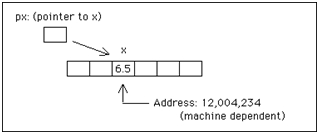
\includegraphics[width=0.5\textwidth]{img/pointer}
\caption{Idea wskaźnika}
\label{fig:wskaznik}
\end{figure}

\begin{example}{[Zastosowania wskaźników]}
W~poniższym przykładzie pokazano kilka możliwości zastosowania wskaźników. Skompilować, zbudować oraz uruchomić przykład.  

\lstinputlisting[caption=Zastosowania wskaźników,style=MyCStyle,label=src:pointer]{src/lab3/pointer.c}

\end{example}

\subsubsection{Tablice}

W~języku C typy danych można umieszczać w~tablicach. Składnia jest przy tym następująca: 

\begin{lstlisting}[style=MyCStyle]
typ nazwatablicy[wymiar];
\end{lstlisting}

W~języku~C tablice zaczynają się od indeksu \lstinline[style=MyCStyle]{0}. Pozostałe elementy zajmują sąsiednie komórki w~pamięci. Język~C traktuje nazwę tablicy jako wskaźnik do jej pierwszego elementu. Tak więc, jeśli \lstinline[style=MyCStyle]{v} jest tablicą, \lstinline[style=MyCStyle]{*v} ma tą samą wartość co element tablicy \lstinline[style=MyCStyle]{v[0]},\lstinline[style=MyCStyle]{*(v+1)} ma tą samą wartość, co element tablicy \lstinline[style=MyCStyle]{v[1]}. Sytuację tę ilustruje rysunek~\ref{fig:tablica}. 

\begin{figure}[!h]
\centering
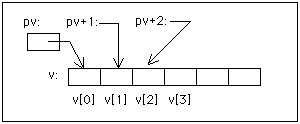
\includegraphics[width=0.5\textwidth]{img/tablica}
\caption{Tablica a~wskaźnika}
\label{fig:tablica}
\end{figure}

Skompilować, zbudować oraz uruchomić przykład. 

\lstinputlisting[caption=Zastosowania wskaźników i~tablic,style=MyCStyle,label=src:table]{src/lab3/table.c}

\subsubsection{Funkcje}

Funkcje w~języku~C pozwalają na znaczne uproszczenie kodów źródłowych. W trakcie laboratorium zetknęliśmy się już z~funkcją główną \lstinline[style=MyCStyle]{main}, a~także z~funkcjami matematycznymi i~funkcjami wejścia/wyjścia. Oprócz zastosowań funkcji bibliotecznych, programista może implementować własne funkcje. Nagłówek i~ciało funkcji mogą przyjąć następującą postać:

\begin{lstlisting}[style=MyCStyle]
typ nazwa_funkcji ( lista_argumentow )
{
	...deklaracja lokalne...

	...operacje...

	return zwracana_wartosc;
}
\end{lstlisting}

Argumenty w~wywołaniach funkcji można przekazywać przez wartość. Oznacza to, że w~ciele funkcji istnieje kopia argumentu wywołania. Jakakolwiek zmiana zmiennej przekazanej do funkcji nie powoduje zmiany wartości zmiennej poza ciałem funkcji. Aby zmienić wartość zmiennej przekazanej w~wywołaniu w~ciele funkcji, należy przekazać ja poprzez wskaźnik. Problem ten ilustrują poniższe przykłady.

\begin{example}{[Przekazywanie argumentów przez wartość]} Skompilować, zbudować oraz uruchomić przykład. 
\lstinputlisting[caption=Przekazywanie argumentów przez wartość,style=MyCStyle,label=src:exchange1]{src/lab3/exchange1.c}
\end{example} 

\begin{example}{[Przekazywanie argumentów przez wskaźnik]} Skompilować, zbudować oraz uruchomić przykład. 
\lstinputlisting[caption=Przekazywanie argumentów przez wskaźnik,style=MyCStyle,label=src:exchange2]{src/lab3/exchange2.c}
\end{example} 

\subsubsection{Przekazywanie argumentów z wiersza poleceń}

Często zdarza się (szczególnie w~systemach UNIX–owych), że argumenty przetwarzane w~programie są przekazywane poprzez wiersz poleceń. Typowe przykłady to \lstinline[style=MyCStyle]{ls -la}, czy też \lstinline[style=MyCStyle]{tail -20}. Argumenty z~wiersza poleceń pozwalają na uzyskanie większej elastyczności naszych programów. Można je przekazywać do programu poprzez funkcję główną \lstinline[style=MyCStyle]{main()}. Ogólna składnia funkcji ma następującą postać: 

\begin{lstlisting}[style=MyCStyle]
main(int argc, char* argv[]);
\end{lstlisting}

gdzie \lstinline[style=MyCStyle]{argc}, określa liczbę argumentów wywołania (łącznie z~nazwą wywoływanego programu), a~\lstinline[style=MyCStyle]{argv} jest tablicą ciągów znakowych \lstinline[style=MyCStyle]{char*}, w~której przechowywane są argumenty wywołania. Sposób użycia ilustruje poniższy przykład.

\begin{example}{[Argumenty wiersza poleceń]} Skompilować, zbudować oraz uruchomić przykład. 
\lstinputlisting[caption=Argumenty wiersza poleceń,style=MyCStyle,label=src:cmd]{src/lab3/cmd.c}
\end{example}

\subsubsection{Operacje I/O (wejścia/wyjścia)}

Język C, poprzez swoje biblioteki, dostarcza różnorodnych funkcji, pozwalających na obsługę wejścia/wyjścia. Na poziomie liter, funkcją która pobiera znak ze standardowego wejścia \lstinline[style=MyCStyle]{stdin}, jest \lstinline[style=MyCStyle]{getchar()}, podczas gdy funkcja \lstinline[style=MyCStyle]{putchar()} zapisuje jeden znak do standardowego wyjścia \lstinline[style=MyCStyle]{stdout}. Użycie funkcji ilustruje poniższy kod źródłowy.

\begin{example}{[Operacje wejścia i~wyjścia]} Skompilować, zbudować oraz uruchomić przykład. 
\lstinputlisting[caption=Użycie funkcji getchar() i putchar(),style=MyCStyle,label=src:io]{src/lab3/io.c}
\end{example}

Znak \lstinline[style=MyCStyle]{EOF} jest wartością końca pliku, zdefiniowaną w~nagłówku biblioteki standardowej. Zakończenie danych (koniec pliku) uzyskujemy poprzez kombinację klawiszy \lstinline[style=MyCStyle]{Ctrl+D}. Bardziej zaawansowaną funkcją pozwalającą pisać sformatowany tekst do standardowego wyjścia jest poznana wcześniej funkcja \lstinline[style=MyCStyle]{printf}. Funkcją, która umożliwia czytanie ze standardowego wejścia jest \lstinline[style=MyCStyle,morekeywords={scanf}]{scanf}. Składnie obu poleceń przedstawiono poniżej.

\begin{lstlisting}[style=MyCStyle,morekeywords={scanf}]
printf("format", zmienne);
scanf("format", &zmienne);
\end{lstlisting}

Odpowiednikiem powyższych wyrażeń, pozwalających pisać do tablic zmiennych typu \lstinline[style=MyCStyle]{char} są poniższe funkcje.

\begin{lstlisting}[style=MyCStyle,morekeywords={scanf,sprintf}]
sprintf(string, "format", zmienne);
sscanf(string, "format", &zmienne);
\end{lstlisting}

String w~składni oznacza nazwę tablicy zmiennych typu \lstinline[style=MyCStyle]{char}, bądź wskaźnik do jej pierwszego elementu.

\subsubsection{Operacje I/O na plikach}

Podobne instrukcje wejścia/wyjścia istnieją w~przypadku obsługi plików. Ogólną składnię I/O w~przypadku plików podano poniżej. 

\begin{lstlisting}[style=MyCStyle]
FILE *fp;			/* wskaznik do pliku */	
fp = fopen(nazwa, tryb);		/* otworzenie pliku */
fscanf(fp, "format", lista_zmiennych);  /* czytanie z pliku */
fprintf(fp, "format", lista_zmiennych);   /* pisanie do pliku */
fclose(fp);		/* zamkniecie pliku */	
\end{lstlisting}

Tryb w~instrukcji \lstinline[style=MyCStyle]{fopen} określa cel otwarcia pliku. Dozwolone tryby przedstawiono w~tabeli~\ref{tab:operacjenaplikach}. 

\begin{table}[h!]
\centering
\caption{Operacje na plikach}
\setlength{\arrayrulewidth}{1pt}
\setlength{\tabcolsep}{6pt}
\renewcommand{\arraystretch}{1.2}
\begin{tabular}{ |p{0.15\textwidth}|p{0.4\textwidth}|}
\hline \rowcolor{gray}
\textbf{Typ} & \textbf{Opis} \\ \hline
\mbox{\lstinline[style=MyBashStyle]{r}} & czytanie z~pliku \\ \hline
\mbox{\lstinline[style=MyBashStyle]{w}} & pisanie do pliku \\ \hline
\mbox{\lstinline[style=MyBashStyle]{a}} & dodanie zawartości do pliku \\ \hline
\end{tabular}
\label{tab:operacjenaplikach}
\end{table}

\begin{example}{[Operacje IO na plikach]} Skompilować, zbudować oraz uruchomić przykład. 
\lstinputlisting[caption=Zastosowanie funkcji fopen() i~fclose(),style=MyCStyle,label=src:iofile]{src/lab3/iofile.c}
\end{example}

\subsection{Ćwiczenia}


%\lstinline[style=MyBashStyle]{}
%\begin{lstlisting}[style=MyBashStyle,caption=Rozbudowany plik Makefile]
%\end{lstlisting}

\begin{myenumerate}
\item Zmodyfikować program obliczający tablicę funkcji \lstinline[style=MyBashStyle]{sinus}, tak, aby zawierał instrukcję sterującą \lstinline[style=MyBashStyle]{for}. Utworzyć funkcję \lstinline[style=MyBashStyle]{sinus} i przenieść jej kod do oddzielnego pliku źródłowego \lstinline[style=MyBashStyle]{sinus.c}. Dołączyć plik nagłówkowy \lstinline[style=MyBashStyle]{sinus.h} z~deklaracją funkcji. Napisać odpowiedni skrypt \lstinline[style=MyBashStyle]{Makefile}. Wyniki zapisać do pliku \lstinline[style=MyBashStyle]{sinus.dat}.
\item Napisz funkcję sprawdzającą ile par liczb całkowitych z przedziału \lstinline[style=MyBashStyle]{<a,b>} jest zawartych w~kole o~średnicy \lstinline[style=MyBashStyle]{8}. ($x^2+y^2\leq 8$). Wartości \lstinline[style=MyBashStyle]{a} i~\lstinline[style=MyBashStyle]{b} powinny być zadawane z klawiatury i przekazywane jako parametry funkcji.
\item Napisać bibliotekę operacji wektorowych, wykorzystując struktury. Zdefiniować wektor jako strukturę:

\begin{lstlisting}[style=MyCStyle]
struct Wektor
{
	double x, y, z;
};
\end{lstlisting}

Biblioteka operacji powinna pozwalać na dodawanie, odejmowanie, mnożenie przez liczbę wektora, liczenie iloczynów skalarnych i~wektorowych. Uzupełnić program  o odpowiednie funkcje testowe.
\item Uzupełnić poprzedni program o operacje transformacji wektorów z układu do układu. Napisać funkcje odpowiadające za elementarne obroty wokół osi \lstinline[style=MyBashStyle]{x}, \lstinline[style=MyBashStyle]{y}, \lstinline[style=MyBashStyle]{z}.
\end{myenumerate}




\cleardoublepage
